\section{Conversion vers la syntaxe abstraite}

\newcommand{\drawcross}[1]{
  \draw[cross] (#1.north west) -- (#1.south east);
  \draw[cross] (#1.north east) -- (#1.south west);
}

\tikzstyle{cross}=[red, very thick]

%--------------expilaction---------------
\subsection{Fonctionnement}
\addtocounter{framenumber}{-1}
\begin{frame}
  \addtocounter{framenumber}{1}
  \frametitle{Syntaxe abstraite\esp}

  \begin{tikzpicture}
    % frame
    \node[frame] (frame) {};
    \tikzstyle{faded}=[draw=black!20,color=black!20]
    
    \node[below=4cm of frame.west, anchor=west, box, faded] (state_1) {\scriptsize Analyse Lexicale};
    \node[right=0.5cm of state_1.east, anchor=west, box, faded] (state_2) {\scriptsize Analyse Syntaxique};
    \node[right=0.5cm of state_2.east, anchor=west, box] (state_3) {\scriptsize Syntaxe Abstraite};
    \node[right=0.5cm of state_3.east, anchor=west, box, faded] (state_4) {\scriptsize Conversion};
    \draw[->, >=latex, faded] (state_1.east) -- (state_2.west);
    \draw[->, >=latex, faded] (state_2.east) -- (state_3.west);
    \draw[->, >=latex, faded] (state_3.east) -- (state_4.west);
    \draw[dashed] (frame.south west) -- (state_3.north west);
    \draw[dashed] (frame.south east) -- (state_3.north east);

    % definition
    \begin{scope}[shift={(-3, 2)}, font=\footnotesize]
      \node (0) at (0, 0) {S};
      \node [below=0.3cm of 0] (1) {A};
      \node [below=0.3cm of 1.south west] (2) {a};
      \node [below=0.3cm of 1.south east] (3) {A};
      \node [below=0.3cm of 3] (4) {B};
      \node [below=0.3cm of 4.south west] (5) {b};
      \node [below=0.3cm of 4.south east] (6) {B};
      \node [below=0.3cm of 6] (7) {$\varepsilon$};

      \draw (0) -- (1);
      \draw (1) -- (2);
      \draw (1) -- (3);
      \draw (3) -- (4);
      \draw (4) -- (5);
      \draw (4) -- (6);
      \draw (6) -- (7);
    
      
      \only<2->{\drawcross{3}}
      \only<3->{\drawcross{6}}
      \only<4->{\drawcross{7}}
      
      \only<5->{
        \node[right=0.8cm of 3, font=\ttfamily] {=>};

        \node [right=2.5cm of 0] (_0) {S};
        \node [below=0.3cm of _0] (_1) {A};
        \node [below=0.3cm of _1.south west] (_2) {a};
        \node [below=0.3cm of _1.south east] (_4) {B};
        \node [below=0.3cm of _4.south] (_5) {b};

        \draw (_0) -- (_1);
        \draw (_1) -- (_2);
        \draw (_1) -- (_4);
        \draw (_4) -- (_5);
      }

      \only<6->{\draw[->, >=latex, draw=blue, very thick] (_4) [bend right] to (_0);}

      \only<7>{
        \node[right=0.8cm of _4, font=\ttfamily] {=>};

        \node [right=2.5cm of _1] (__0) {S};
        \node [below=0.3cm of __0.south west] (__1) {A};
        \node [below=0.3cm of __1.south] (__2) {a};
        \node [below=0.3cm of __0.south east] (__4) {B};
        \node [below=0.3cm of __4.south] (__5) {b};

        \draw (__0) -- (__1);
        \draw (__1) -- (__2);
        \draw (__0) -- (__4);
        \draw (__4) -- (__5);
        }
    \end{scope}

  \end{tikzpicture}

\end{frame}

%----------un exemple----------
\addtocounter{framenumber}{-1}
\subsection{Un exemple}
\begin{frame}
  \addtocounter{framenumber}{1}
  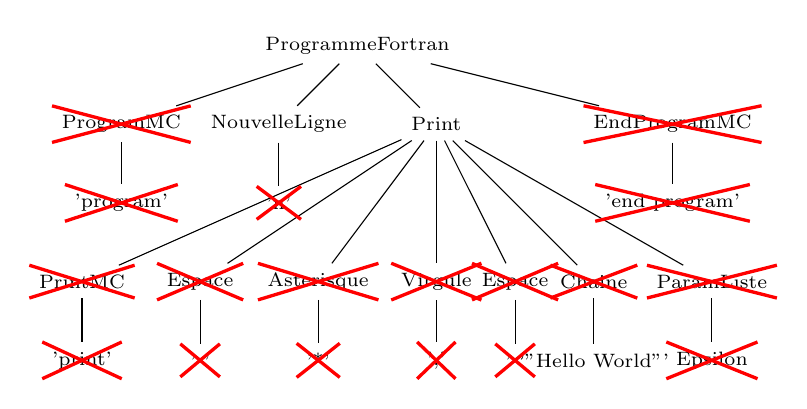
\begin{tikzpicture}
    \begin{scope}
      \node{};
    \end{scope}
    \begin{scope}[shift={(2, 0)}]
      \node[font=\scriptsize] (0) at (-3, 0) {ProgrammeFortran};
  
      \node[font=\scriptsize] (1) at (-6, -1) {ProgramMC};
      \node[font=\scriptsize] (2) at (-4, -1) {NouvelleLigne};
      \node[font=\scriptsize] (3) at (-2, -1) {Print};
      \node[font=\scriptsize] (4) at (1, -1) {EndProgramMC};
      
      \node[font=\scriptsize] (5) at (-6, -2) {'program'};
      \node[font=\scriptsize] (6) at (-4, -2) {'\\n'};
      \node[font=\scriptsize] (7) at (-6.5, -3) {PrintMC};
      \node[font=\scriptsize] (8) at (-5, -3) {Espace};
      \node[font=\scriptsize] (9) at (-3.5, -3) {Asterisque};
      \node[font=\scriptsize] (10) at (-2, -3) {Virgule};
      \node[font=\scriptsize] (11) at (-1, -3) {Espace};
      \node[font=\scriptsize] (12) at (0, -3) {Chaine};
      \node[font=\scriptsize] (13) at (1.5, -3) {ParamListe};
      \node[font=\scriptsize] (14) at (1, -2){'\lin{end} program'};
      
      \node[font=\scriptsize] (15) at (-6.5, -4) {'print'};
      \node[font=\scriptsize] (16) at (-5, -4) {' '};
      \node[font=\scriptsize] (17) at (-3.5, -4) {'*'};
      \node[font=\scriptsize] (18) at (-2, -4) {','};
      \node[font=\scriptsize] (19) at (-1, -4) {' '};
      \node[font=\scriptsize] (20) at (0, -4) {'"Hello World"'};
      \node[font=\scriptsize] (21) at (1.5, -4) {Epsilon};
    \end{scope}
    
    \draw (0) -- (1);
    \draw (0) -- (2);
    \draw (0) -- (3);
    \draw (0) -- (4);

    \draw (1) -- (5);
    \draw (2) -- (6);
    \draw (3) -- (7);
    \draw (3) -- (8);
    \draw (3) -- (9);
    \draw (3) -- (10);
    \draw (3) -- (11);
    \draw (3) -- (12);
    \draw (3) -- (13);
    \draw (4) -- (14);
    
    \draw (7) -- (15);
    \draw (8) -- (16);
    \draw (9) -- (17);
    \draw (10) -- (18);
    \draw (11) -- (19);
    \draw (12) -- (20);
    \draw (13) -- (21);

    \only<2>{
      \drawcross{1}
      \drawcross{5}
      \drawcross{6}
      \drawcross{7}
      \drawcross{15}
      \drawcross{8}
      \drawcross{16}
      \drawcross{9}
      \drawcross{17}
      \drawcross{11}
      \drawcross{19}
      \drawcross{13}
      \drawcross{21}
      \drawcross{4}
      \drawcross{14}
      \drawcross{10}
      \drawcross{18}
      \drawcross{12}
    }
  \end{tikzpicture}

\end{frame}

\begin{frame}
  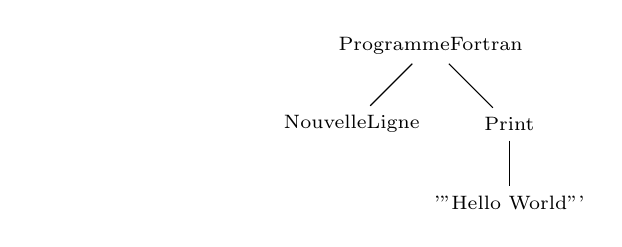
\begin{tikzpicture}
    \begin{scope}
      \node{};
    \end{scope}
    \begin{scope}[shift={(5, 0)}]
      \node[font=\scriptsize] (0) at (0, 0) {ProgrammeFortran};
      \node[font=\scriptsize] (1) at (-1, -1) {NouvelleLigne};
      \node[font=\scriptsize] (2) at (1, -1) {Print};
      \node[font=\scriptsize] (3) at (1, -2) {'"Hello World"'};
    \end{scope}
    
    \draw (0) -- (1);
    \draw (0) -- (2);
    \draw (2) -- (3);
  \end{tikzpicture}

\end{frame}